%!TEX program=xelatex
\documentclass[10pt, a4paper, twocolumn]{article}
\usepackage[margin=2.5cm]{geometry}
\setlength\columnsep{0.5cm}
\linespread{1}
\usepackage[]{authblk}

% chinese font (CISC template): prefer bundled kaiu.ttf; fallback for machines without it
\usepackage{fontspec}
\usepackage{xeCJK}
\IfFileExists{kaiu.ttf}{%
  \setCJKmainfont[AutoFakeBold=2,AutoFakeSlant=.4]{[kaiu.ttf]}%
}{%
  \setCJKmainfont{Kaiti SC}[AutoFakeBold=2,AutoFakeSlant=.4]%
}%
\setmainfont{Times New Roman}

\usepackage{titlesec}

\titleformat{\section}
  {\fontsize{12pt}{15}\bfseries}{\thesection}{1em}{}
\titleformat{\subsection}
 {\fontsize{11pt}{15}\bfseries}{\thesubsection}{1em}{}
  \titleformat{\subsubsection}
 {\fontsize{11pt}{15}\bfseries}{\thesubsubsection}{1em}{}

\renewcommand\thesection{\arabic{section}.}
\renewcommand\thesubsection{\thesection\arabic{subsection}}
\renewcommand\thesubsubsection{\thesubsection.\arabic{subsubsection}}

\usepackage[font={bf}, labelsep=space]{caption}
\usepackage{graphicx}
\usepackage{url}
\usepackage{booktabs}
\usepackage{tabularx}
\usepackage{amsmath}
\usepackage{indentfirst}

\graphicspath{{figures/}}

\renewcommand{\abstractname}{摘要}
\renewcommand{\refname}{參考文獻}
\renewcommand{\figurename}{圖}
\renewcommand{\tablename}{表}

% abstract (CISC template)
\usepackage{abstract}
\renewcommand{\abstractnamefont}{\fontsize{12pt}{15}\bfseries}
\renewcommand{\abstracttextfont}{\fontsize{10pt}{15}}
\setlength{\absleftindent}{0pt}
\setlength{\absrightindent}{0pt}

\date{}
\begin{document}
\title{\fontsize{16pt}{1}\selectfont\textbf{From Encrypted Flows to Security Event Signals: An Edge-Native Pipeline for Threat-Aware Traffic Analysis}}

\author[1]{Yu-Lun Tsai}
\author[1]{Yu-Liang Cheng}
\author[1]{Yu-Ying Huang}
\author[1]{Ching-Hao Mao}
\affil[1]{Bachelor's Program in Artificial Intelligence and Information Security, Fu Jen Catholic University, New Taipei City, Taiwan}
\affil[1]{\texttt{412580084@cloud.fju.edu.tw} (Y.-L. Tsai);\quad \texttt{412580292@cloud.fju.edu.tw} (Y.-L. Cheng);\quad \texttt{412580060@cloud.fju.edu.tw} (Y.-Y. Huang);\quad \texttt{chmao2008@gmail.com} (C.-H. Mao)}
\renewcommand{\Affilfont}{\fontsize{12pt}{1}\bfseries}
\renewcommand{\Authfont}{\fontsize{12pt}{1}\bfseries}
\renewcommand\Authand{, }
\setlength{\affilsep}{1mm}

\maketitle
\pagestyle{empty}
\thispagestyle{empty}
\begin{abstract}
Widespread HTTPS/TLS limits cleartext visibility at enterprise and carrier edges, so operators must infer risk from flow-level metadata, timing, and side-channel structure rather than payloads.
Encrypted traffic classifiers frequently report a single label or score vector, yet security operations increasingly require \emph{structured security event signals}: versioned records that bind identity, network context, calibrated model output, threat semantics, and provenance for correlation, ticketing, and later reasoning.

This paper is \emph{not} a study of a specific vendor telemetry product nor a contest among neural encoders; it examines how encrypted flow-level predictions can be \emph{transformed} into threshold-consistent, schema-stable events suitable for edge-native defense stacks.
We instantiate a two-stage pipeline: Stage~1 benign/malicious screening with calibrated dispatch, then Stage~2 threat-behavior labeling on the admitted subset, each flow emitting a normalized record spanning identity, context, scores, semantics, and governance fields.

\textbf{Validated snapshot:} Stage~1 out-of-distribution (OOD) macro-F1 is $0.9478$; Stage~2 macro-F1 is $0.7778$ on the documented held-out split; replaying $460$ flows yields $460$ event signals with $42$ flows admitted to Stage~2 under the deployed threshold policy.
We position this work as an \emph{initial validated input layer}---not a complete automated threat reasoning or response system; episode analytics, trust inference, and AI-assisted triage remain downstream consumers.

\newline
\textbf{關鍵字:} TLS/HTTPS, encrypted traffic, security event signal, edge defense, two-stage classification, operational validation.
\end{abstract}

\section{Introduction}
\label{sec:intro}

Enterprise, cloud, and industrial edges now carry predominantly encrypted sessions.
Where bulk decryption is infeasible or policy-disallowed, defenders observe TLS handshakes, record sizes, inter-arrival times, and coarse metadata---signals that are legally and technically accessible but weakly aligned with traditional application-layer antivirus taxonomies.

\textbf{Gap.}
A rich literature improves \emph{encrypted traffic classification}, yet many published systems stop at an argmax label.
In contrast, SOCs, incident responders, and orchestration fabrics consume \emph{events}: artifacts with stable identifiers, timestamps, observable context, calibrated confidence, tactic-relevant semantics, and lineage to models and datasets.
Without such structure, classifiers are hard to replay after model updates, difficult to correlate across hosts, and risky to feed into automated playbooks.

\textbf{Positioning.}
We treat the learning stack as \emph{replaceable}: commodity flow export (e.g., IPFIX-style summaries~\cite{rfc7011}) and learned representations~\cite{lin2022etbert} are implementation details behind a fixed \emph{event interface}.
Our scientific question is operational: \emph{How should encrypted flow predictions be serialized so training-time validation, online inference, and offline replay agree on dispatch and final fields?}

\textbf{Approach.}
Stage~1 performs benign/malicious screening with probability calibration and a single validated threshold policy shared across train, serve, and replay.
Stage~2 assigns finer threat-behavior semantics only to flows that satisfy that gate, reflecting asymmetric compute budgets at the edge.
Each flow maps to the schema in Section~\ref{sec:design}.

\textbf{Snapshot.}
Stage~1 OOD macro-F1 is $0.9478$; Stage~2 macro-F1 is $0.7778$; $460$ replayed flows produce $460$ structured signals with $42$ Stage~2 inferences, matching dispatch counters under fixed versions.

\paragraph{Contributions.}
\begin{itemize}\itemsep1pt
  \item \textbf{Two-stage edge screening and behavior labeling} with explicitly shared calibration/threshold semantics between training and production.
  \item \textbf{Structured event-signal schema} aligning inference outputs to downstream correlation and CTI-style fields without vendor lock-in.
  \item \textbf{Replay validation} demonstrating per-flow signal cardinality and Stage~1/Stage~2 admission parity on archived traces.
\end{itemize}

Temporal feature fusion, open-set discovery, long-term drift adaptation, unseen-protocol guarantees, Edge-SLM copilots, and automated enforcement are \emph{explicitly out of scope} for the present validation (Section~\ref{sec:conclusion}).

\section{Related Work}
\label{sec:related}

\subsection{Encrypted traffic classification}

Survey literature classifies encrypted flows using handcrafted statistics, deep models over bytes or bursts, and learned sequence encoders~\cite{aceto2019mobile}.
Pre-training followed by fine-tuning improves sample efficiency and transfer across tasks~\cite{lin2022etbert,zhou2025trafficformer}.
These works advance \emph{representation quality}; our focus is instead the \emph{operational envelope}: converting model outputs into auditable security events.

\subsection{Evaluation practice and robustness}

Encrypted classifiers are sensitive to dataset provenance, split protocols, and environment shifts~\cite{wickramasinghe2025sok}.
Noisy labels and scarce malicious HTTPS traces complicate training~\cite{qing2024rapier}; robustness studies highlight performance collapse under dynamic network conditions~\cite{qing2025dynamic}.
Our evaluation therefore reports an OOD test draw with zero cross-split group overlap for Stage~1 and complements classifier metrics with threshold-consistent replay.

\subsection{Semantics, telemetry export, and security events}

Flow and session records are routinely exported using standard IPFIX-style fields for analytics pipelines~\cite{rfc7011}.
Downstream reasoning benefits when events align to shared threat semantics (MITRE ATT\&CK, STIX) for correlation~\cite{mitre2025attack,oasis2020stix}.
We bridge these threads: encrypted-flow inference is treated as an \emph{upstream producer} of STIX-amenable records, not as a stand-alone classifier leaderboard entry.

\section{System Design}
\label{sec:design}

This section states the engineering contract for an edge-native pipeline: what problem we solve, how layers compose from observations to serialized events, and which labels and schema fields downstream tools may rely on.

\subsection{Goals and Problem Statement}

Edge-native defenses must (i)~operate without payload visibility, (ii)~emit machine-readable evidence richer than a scalar label, and (iii)~allow telemetry ingress and model backbones to evolve without breaking downstream automation.
We pose:
\begin{quote}\small
\emph{Given an encrypted flow observed at the edge, how can a two-stage inference cascade convert it into a threshold-consistent and semantically meaningful security event signal?}
\end{quote}

\textbf{Non-goals.}
We do \emph{not} claim full episode reconstruction, global trust calibration, automated containment, or conversational triage; those modules consume---but lie outside---the validated artifact.

\subsection{Pipeline Overview}

Figure~\ref{fig:system_overview} situates four layers.
\textbf{Layer~0} aggregates heterogeneous observations: programmable telemetry, gateways, SPAN/mirror ports, curated public captures, and controlled HTTPS/TLS threat scenarios.
\textbf{Layer~1} builds flow records: five-tuple, timing, optional TLS metadata, sequences of lengths/directions/inter-arrival times (for future temporal models), and lineage fields (collection run, dataset id).
\textbf{Layer~2} runs Stage~1 screening and Stage~2 behavior classification under a shared dispatch policy (Section~\ref{sec:method}).
\textbf{Layer~3} materializes the event tuple with checksums, schema/model versions, and consumer hooks.

\begin{figure*}[t]
  \centering
  \IfFileExists{figures/system_overview.pdf}{%
    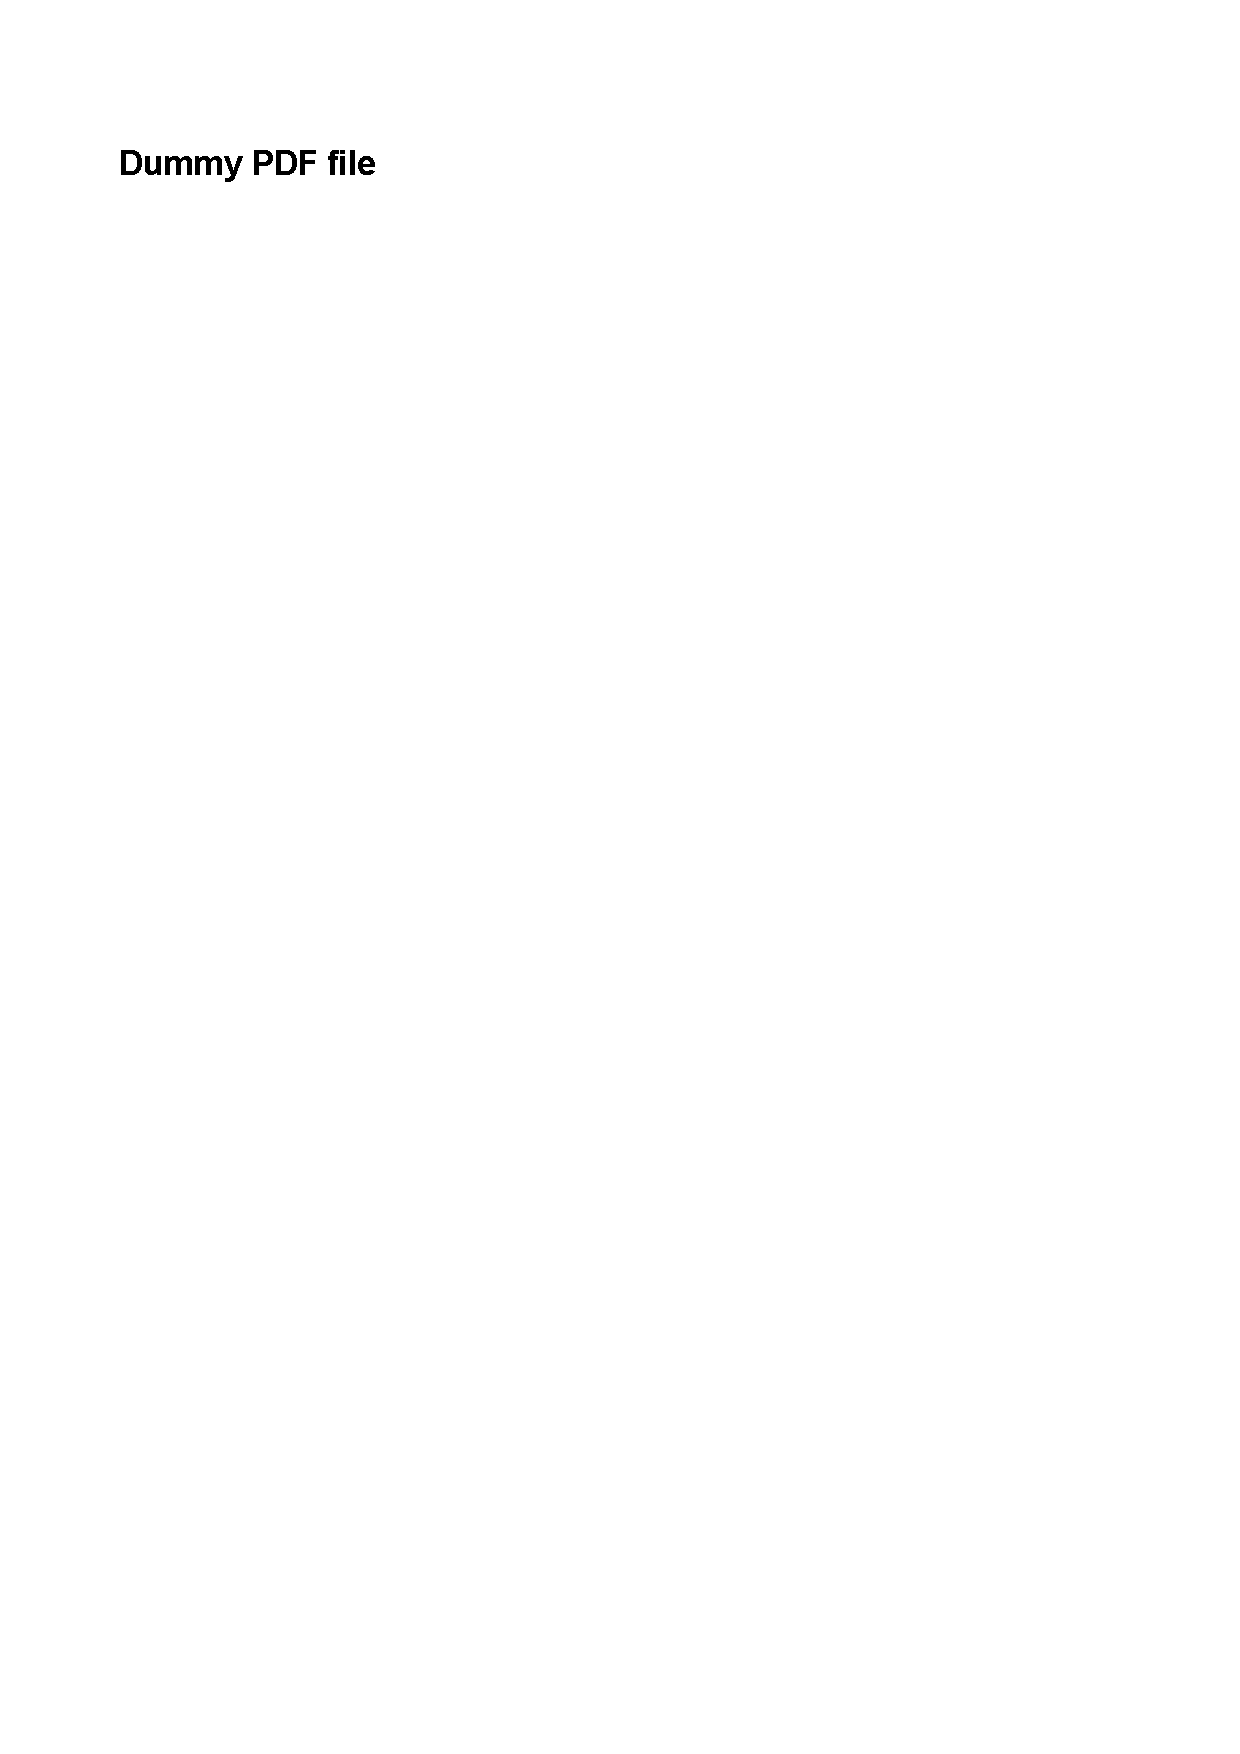
\includegraphics[width=0.96\textwidth]{system_overview}%
  }{%
    \fbox{%
      \begin{minipage}{0.94\textwidth}\footnotesize\centering
        \textbf{L0} edge sources (telemetry, gateways, mirrors, public + synthetic TLS data)\\[1mm]
        $\Downarrow$\quad \textbf{L1} flow assembly + provenance\\[1mm]
        $\Downarrow$\quad \textbf{L2} Stage~1 screening $\rightarrow$ threshold dispatch $\rightarrow$ Stage~2 behavior labels\\[1mm]
        $\Downarrow$\quad \textbf{L3} normalized security event signal (IDs, context, scores, semantics, governance)
      \end{minipage}}%
  }
  \caption{Edge-native pipeline from encrypted observations to structured event signals (artwork may be replaced).}
  \label{fig:system_overview}
\end{figure*}

\subsection{Threat-behavior label space}

Table~\ref{tab:label_space} lists the validated taxonomy.
Stage~1 isolates malicious candidates; Stage~2 attaches analyst-facing behavior semantics closer to SOC vocabulary than raw application IDs.

\begin{table}[t]
  \centering
  \caption{Two-stage label contract (validated scope).}
  \label{tab:label_space}
  \footnotesize
  \setlength{\tabcolsep}{3pt}
  \begin{tabular}{@{}lp{0.38\linewidth}@{}}
    \toprule
    Stage / label & Role \\
    \midrule
    Stage~1 benign / malicious & Screening + dispatch gate \\
    Stage~2 C2 & Suspicious control channel semantics \\
    Stage~2 data exfiltration & Abnormal outbound movement semantics \\
    Stage~2 HTTPS tunneling & Covert channel over web TLS \\
    Stage~2 domain-fronting-like & Destination-obfuscation semantics \\
    \bottomrule
  \end{tabular}
\end{table}

\subsection{Event signal schema}

Equation~\eqref{eq:event} summarizes the informational bundles embedded in each record; Table~\ref{tab:event_schema} enumerates representative keys consumed by downstream SIEM/SOAR adapters.
\begin{equation}
  e_i = \{m_i, n_i, x_i, c_i, a_i, g_i\}.
  \label{eq:event}
\end{equation}
$m_i$ covers identifiers and timestamps; $n_i$ network context; $x_i$ optional feature sequences reserved for temporal extensions; $c_i$ calibrated Stage~1/Stage~2 outputs; $a_i$ tactic/technique hooks; $g_i$ dataset + schema/model hashes.

\begin{table*}[t]
  \centering
  \caption{Representative security event signal field groups.}
  \label{tab:event_schema}
  \footnotesize
  \setlength{\tabcolsep}{3pt}
  \begin{tabularx}{\textwidth}{@{}l >{\raggedright\arraybackslash}X@{}}
    \toprule
    Group & Examples (non-exhaustive) \\
    \midrule
    Identity / time & \texttt{event\_id}, \texttt{flow\_id}, \texttt{session\_id}, \texttt{event\_time}, \texttt{run\_id} \\
    Network context & \texttt{src\_ip}, \texttt{dst\_ip}, ports, \texttt{protocol}, logical zones \\
    Sequences (optional) & \texttt{packet\_len\_seq}, \texttt{direction\_seq}, \texttt{iat\_seq} \\
    Inference & \texttt{stage1\_label}, \texttt{stage1\_score}, \texttt{stage2\_label}, \texttt{stage2\_score}, \texttt{dispatch\_reason} \\
    Threat semantics & \texttt{threat\_behavior}, \texttt{tactic}, \texttt{technique}, \texttt{stix\_mapping} \\
    Governance & \texttt{schema\_version}, \texttt{model\_version}, \texttt{dataset\_source}, content checksum \\
    Downstream hooks & \texttt{consumer\_hint}, \texttt{replay\_id}, ticket or playbook placeholders \\
    \bottomrule
  \end{tabularx}
\end{table*}

Designated fields ensure replay can assert bit-identical serialization when inputs and configuration versions match---a requirement for regression testing gateways and analytics rules.

\section{Methodology}
\label{sec:method}

This section instantiates the design of Section~\ref{sec:design}: how features are produced, how Stage~1/Stage~2 models are trained under a single dispatch policy, and how outputs are serialized and replay-checked against that policy.

\subsection{Feature materialization}

We ingest any source honoring the Layer~1 contract (Section~\ref{sec:design}): flows keyed by five-tuple and time window, augmented with TLS metadata when present and optional per-packet summaries for future temporal modules.
Feature dictionaries are versioned; hashes over canonicalized tensors are stored in $g_i$ to detect silent skew between training and serving.

\subsection{Stage~1 screening and calibration}

The Stage~1 classifier outputs malicious probability $\hat{p}$; temperature scaling (or equivalent) maps logits to calibrated $\bar{p}$ on a held-out development split disjoint from OOD evaluation.
Class imbalance is countered via reweighting or balanced sampling; the objective is reliable ranking at the operating threshold rather than leaderboard accuracy alone.

\subsection{Threshold-consistent dispatch}

Let $\tau$ denote the malicious admission threshold selected on development replay traces.
A flow escalates iff $\bar{p}_{\mathrm{mal}} \ge \tau$.
The \emph{same} inequality governs (i)~mining supervisory tuples for Stage~2 training, (ii)~online inference, and (iii)~offline archival replay.
This alignment prevents benign label drift (e.g., exporting ``malicious'' nominal labels while dispatch logic suppresses Stage~2) and is necessary for faithful event emission.

\subsection{Stage~2 behavior model}

Stage~2 is trained exclusively on flows whose features were generated under the dispatch gate, mirroring conditional distributions at deployment.
The classifier head targets the Stage~2 taxonomy in Table~\ref{tab:label_space}; macro-F1 is emphasized due to class imbalance.

\subsection{Signal synthesis and replay}

For each flow we populate $e_i$ (Eq.~\eqref{eq:event}) including top-$k$ logits, calibrated scores, boolean dispatch flags, schema/model version tuples, and deterministic checksums of serialized inputs.
Replay replays stored features through the frozen cascade; Section~\ref{sec:experiments} verifies one signal per ingested flow and identical Stage~2 cardinality relative to admitted malicious traffic.

\section{Experimental Validation}
\label{sec:experiments}

\subsection{Objectives}

We answer three validation questions aligned with the event-signal thesis:
\begin{itemize}\itemsep1pt
  \item \textbf{RQ1:} Under strict group isolation, does Stage~1 retain strong OOD macro-F1 suitable for dispatch?
  \item \textbf{RQ2:} On held-out malicious-focused data, does Stage~2 retain non-trivial macro-F1 despite class imbalance?
  \item \textbf{RQ3:} Does replay reproduce one event signal per input flow with consistent Stage~1/Stage~2 admission?
\end{itemize}
Success means downstream consumers can trust serialized fields---not that the pipeline autonomously contains incidents.

\subsection{Data and protocol}

Evaluations fuse controlled laboratory HTTPS/TLS scenarios with public encrypted-traffic corpora (tunneling, DNS-over-HTTPS families, etc.).
Stage~1 estimates benign vs.\ malicious propagation with train/dev/test sizes $(4160,450,460)$, class ratio $3744{:}416$ on training, and \emph{zero} split-group overlap---reducing leakage from correlated captures.
Stage~2 trains on dispatched flows with split $(414,88,93)$; test support per behavior is $(20,14,45,14)$ for C2, data exfiltration, HTTPS tunneling, and domain-fronting-like classes respectively.

All numbers below are \emph{frozen} artifact exports; we do not claim adaptive drift handling or open-set guarantees.

\subsection{Results and interpretation}

Table~\ref{tab:validation} aggregates headline metrics.
Stage~1 achieves \textbf{0.9478} OOD macro-F1, supporting its role as a conservative yet informative gate: analysts receive calibrated context even when flows stay benign, while suspicious flows accumulate structured evidence.

Stage~2 reaches \textbf{0.8495} accuracy and \textbf{0.7778} macro-F1 on $n=93$.
Macro-F1 reflects imbalance; accuracy complements readability but should not be interpreted as operational utility in isolation.
These metrics validate \emph{behavior tagging conditioned on dispatch}, not end-to-end investigative conclusions.

Replay exercises the full serialization path: \textbf{460} ingested flows yield \textbf{460} signals; Stage~1 tallies \textbf{418} benign vs.\ \textbf{42} malicious calls, and all \textbf{42} malicious flows invoke Stage~2---demonstrating parity between scoring, dispatch booleans, and serialized event fields.
Discrepancies here would break SOAR automations; their absence supports the engineering thesis of threshold-consistent events.

\subsection{Limitations}

We do not evaluate long-horizon temporal fusion, earliest-prefix decisions, continual learning under concept drift, or detection of entirely novel threat families.
Nor do we study Edge-hosted large language models or automated blocking policies consuming these signals.
Those directions require consumers and safeguards beyond the scope of this input-layer validation.

\begin{table*}[t]
  \centering
  \caption{Validated experimental snapshot (counts are flows unless noted).}
  \label{tab:validation}
  \footnotesize
  \setlength{\tabcolsep}{4pt}
  \begin{tabular}{@{}p{0.28\textwidth} p{0.66\textwidth}@{}}
    \toprule
    Item & Value \\
    \midrule
    Stage~1 train / dev / test & 4160 / 450 / 460 \\
    Stage~1 train benign:malicious & 3744 : 416 \\
    Stage~1 group overlap (train--dev--test) & 0 \\
    Stage~1 OOD macro-F1 (test) & 0.9478 \\
    \midrule
    Stage~2 train / dev / test & 414 / 88 / 93 \\
    Stage~2 test accuracy / macro-F1 & 0.8495 / 0.7778 \\
    Stage~2 test support by class$^{\dagger}$ & 20 / 14 / 45 / 14 \\
    \midrule
    Replay flows / emitted event signals & 460 / 460 \\
    Replay Stage~1 benign / malicious & 418 / 42 \\
    Replay flows entering Stage~2 & 42 \\
    \bottomrule
  \end{tabular}\\[-2pt]
  {\footnotesize $^{\dagger}$C2, data exfiltration, HTTPS tunneling, domain-fronting-like.}
\end{table*}


\section{Conclusion}
\label{sec:conclusion}

This paper argued that encrypted threat analysis at the edge should deliver \emph{structured, threshold-consistent security event signals}, not isolated classifier outputs.
We presented a two-stage, vendor-neutral pipeline: calibrated Stage~1 screening, conditional Stage~2 behavior labeling, and deterministic serialization aligned with SOC-oriented schema elements.
Validated evidence includes Stage~1 OOD macro-F1 \textbf{0.9478}, Stage~2 macro-F1 \textbf{0.7778}, and replay coverage showing \textbf{460} flows $\rightarrow$ \textbf{460} signals with \textbf{42} Stage~2 inferences---confirming dispatch-aligned event generation.

The contribution is intentionally narrow: an \textbf{initial input layer} for correlation, ticketing, and future reasoning modules.
Realizing trustworthy episode analytics, open-world robustness, temporal fusion, Edge-SLM copilots, or automated enforcement demands additional science and governance; this work supplies the normalized event substrate on which those systems can build without re-deriving per-flow semantics from raw telemetry on every iteration.


\bibliography{reference}
\bibliographystyle{abbrv}

\end{document}

% Format from CISC2026_format_XeLaTeX.tex; modular layout: sections/, figures/, tables/, reference.bib
